\section{Duże bitmapy}
\label{sec:duze-bitmapy}

Rozdział sprawdza, jak obie reguły radzą sobie ze zdjęciami kotów o $N = \num{60000}$ pikseli (rozdział~\ref{sec:zbiory-dodatkowe}), i podaje czas oraz pamięć potrzebne do uczenia i odtwarzania. Wykorzystano eksperymenty \texttt{cats-noise}, \texttt{cats-occlusion} i \texttt{benchmark} z Tabeli~\ref{tab:eksperymenty}.

\subsection{Stabilność wzorców}
\label{sec:duze-stabilnosc}

Reguła Oji stabilizuje wszystkie 12 zdjęć w obu zbiorach, a reguła Hebba tylko 2 zdjęcia zbioru \texttt{cats-300x200-median} i 8 zdjęć zbioru \texttt{cats-300x200-dither}. Niestabilne piksele zbioru median pokazano na Rysunku~\ref{fig:koty-niestabilne}. Obciążenie $p/N = \num{2e-4}$ jest wielokrotnie mniejsze niż granica \num{0.138} dla wzorców losowych, więc o niepowodzeniu reguły Hebba decydują korelacje zdjęć, a nie ich liczba. Suma $\sum_{\mu \ne \nu} \lvert m^{\mu\nu} \rvert$ nakładań jednego zdjęcia z pozostałymi wynosi od \num{0.85} do \num{2.32} w zbiorze median i od \num{0.18} do \num{1.59} w zbiorze dither. Warunek wystarczający z rozdziału~\ref{sec:regula-hebba}, czyli suma mniejsza niż $1 - p/N$, jest spełniony dokładnie dla tych zdjęć, które są stabilne. Zbiór dither ma mniejsze nakładania i dlatego więcej stabilnych wzorców, mimo że udział czarnych pikseli jest w nim bardziej nierówny (Tabela~\ref{tab:zbiory}).

\begin{figure}[H]
    \centering
    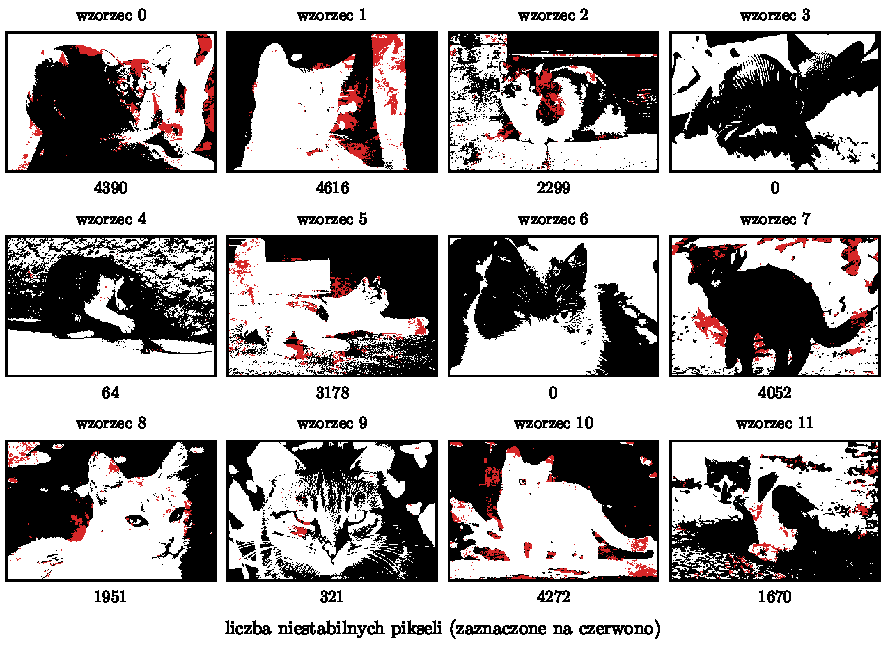
\includegraphics[width=0.8\textwidth]{cats-noise/figures/unstable-median-hebb.pdf}
    \caption{Niestabilne piksele zdjęć zbioru \texttt{cats-300x200-median} przy regule Hebba (zaznaczone na czerwono) i ich liczba pod każdym zdjęciem.}
    \label{fig:koty-niestabilne}
\end{figure}

\noindent Pola wyrównane reguły Hebba są ujemne w \qty{3.7}{\percent} pikseli zbioru median i w \qty{0.73}{\percent} pikseli zbioru dither, a najmniejsze wynoszą $\num{-1.32}$ i $\num{-0.59}$. Przy regule Oji wszystkie pola wyrównane leżą między \num{0.9995} a \num{0.9999}, czyli $h \approx P \xi = \xi$, zgodnie z rozdziałem~\ref{sec:regula-oji}. Uczenie trwało 356 epok dla zbioru median i 226 epok dla zbioru dither.

\subsection{Odzyskiwanie}
\label{sec:duze-odzyskiwanie}

Odsetek odzyskań przy odwróceniu losowych pikseli pokazano na Rysunku~\ref{fig:koty-szum}. Przy regule Hebba aż do szumu \num{0.4} różni się on od odsetka stabilnych wzorców najwyżej o \num{0.009}, czyli sieć odzyskuje stabilne zdjęcia prawie zawsze, a niestabilnych nigdy. Niestabilne zdjęcia kończą w stanach pozornych, a średnie nakładanie stanu końcowego z celem wynosi dla nich około \num{0.5}. Reguła Oji odzyskuje każde zdjęcie aż do szumu \num{0.45}, zawsze w jednym kroku. Pole $h$ jest wtedy z dokładnością do przekątnej rzutem wejścia na podprzestrzeń 12 wzorców. Odwrócone piksele leżą prawie całkowicie poza tą podprzestrzenią, więc rzut ma w każdym pikselu znak celu (wyprowadzenie własne). Przy szumie \num{0.5} wejście nie niesie informacji o celu i odzyskań nie ma.

\begin{figure}[H]
    \centering
    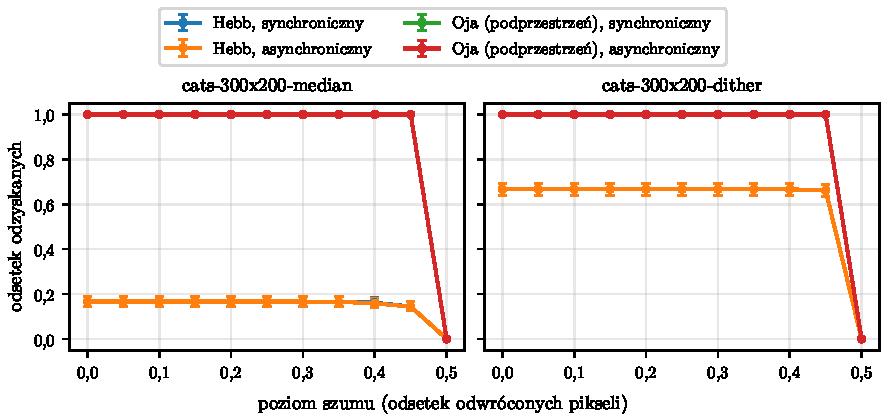
\includegraphics[width=0.75\textwidth]{cats-noise/figures/recovery.pdf}
    \caption{Odsetek odzyskanych wzorców w zależności od poziomu szumu dla zdjęć kotów (100 prób na wzorzec, słupki to 95-procentowe przedziały Wilsona).}
    \label{fig:koty-szum}
\end{figure}

\noindent Klasy stanów końcowych przy zasłonięciu pokazano na Rysunku~\ref{fig:koty-zasloniecie}. Reguła Hebba traci przy zasłonięciu także część stabilnych zdjęć. W zbiorze median przy zasłonięciu \num{0.3} odsetek odzyskań wynosi \num{0.101} w trybie synchronicznym, wobec \num{0.167} przy tym samym poziomie szumu. Reguła Oji odzyskuje co najmniej \qty{90}{\percent} zdjęć median do zasłonięcia \num{0.6} i ponad połowę jeszcze przy \num{0.8}, a zdjęć dither odpowiednio do \num{0.4} i \num{0.5}.

\begin{figure}[H]
    \centering
    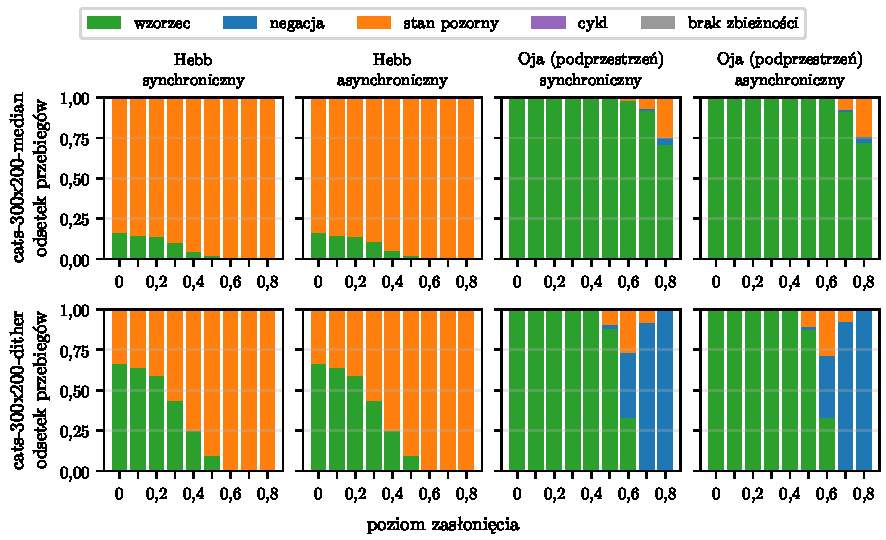
\includegraphics[width=0.9\textwidth]{cats-occlusion/figures/classes.pdf}
    \caption{Klasy stanów końcowych w zależności od poziomu zasłonięcia dla zdjęć kotów. Górne wykresy: zbiór \texttt{cats-300x200-median}. Dolne wykresy: zbiór \texttt{cats-300x200-dither}.}
    \label{fig:koty-zasloniecie}
\end{figure}

\noindent Przy regule Oji w zbiorze dither od zasłonięcia \num{0.7} prawie wszystkie przebiegi kończą w negacji. W obu trybach łącznie w \num{2022} z \num{2190} takich przebiegów przy \num{0.7} i we wszystkich przy \num{0.8} jest to negacja wzorca 1. Wzorzec 1 jest najciemniejszym zdjęciem zbioru (\qty{81.7}{\percent} pikseli czarnych), więc jego negacja jest prawie cała biała, tak jak pas zasłonięcia. Dla \qty{88.8}{\percent} możliwych położeń pasa przy zasłonięciu \num{0.7} i dla wszystkich przy \num{0.8} zasłonięte wejście ma największe nakładanie właśnie z $-\xi^1$, a nie z celem.

Przebieg odtwarzania jednego zdjęcia z połową zasłoniętych wierszy pokazano na Rysunku~\ref{fig:koty-przebieg}, a przebieg reguły Hebba także w przeglądarce na Rysunku~\ref{fig:przegladarka}. Przy regule Hebba sieć po 10 krokach kończy w stanie pozornym, którego nakładanie z celem wynosi tylko \num{0.396}, a ze wzorcem 10 aż \num{0.665}. Reguła Oji odtwarza cel po 2 krokach, a energia końcowa $\num{-29993.87}$ jest bliska najmniejszej energii $-(N - r)/2 = \num{-29994}$ z~\eqref{eq:energia-rzut} dla $r = 12$.

\begin{figure}[H]
    \centering
    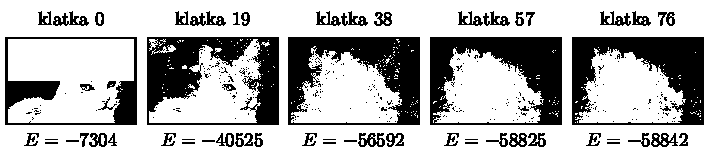
\includegraphics[width=0.8\textwidth]{cats-occlusion/figures/recall-occlusion-hebb.pdf}

    \vspace{0.2cm}
    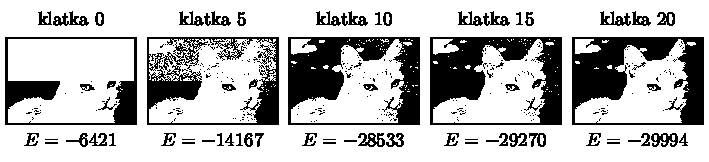
\includegraphics[width=0.8\textwidth]{cats-occlusion/figures/recall-occlusion-oja.pdf}
    \caption{Odtwarzanie wzorca 8 zbioru \texttt{cats-300x200-median} z wejścia z zasłoniętymi 100 wierszami (tryb asynchroniczny, klatka co \num{6000} aktualizacji). Górny wykres: reguła Hebba. Dolny wykres: reguła Oji.}
    \label{fig:koty-przebieg}
\end{figure}

\subsection{Czas i pamięć}
\label{sec:czas-pamiec}

Czas i pamięć uczenia oraz odtwarzania zmierzono dla 12 losowych wzorców przy $N$ od \num{1024} do \num{60000} i dla obu zbiorów kotów (Rysunek~\ref{fig:benchmark}). Każda wartość to mediana z 5 powtórzeń na komputerze z procesorem Intel Core i5-1145G7 (8 wątków) i \qty{15.4}{GB} pamięci RAM. Wagi gęste zajmują dokładnie $8N^2$ bajtów, więc pomiary wag gęstych zakończono przy $N = \num{16384}$ (\qty{2}{GiB}). Przy $N = \num{60000}$ potrzebowałyby \qty{26.8}{GiB}, czyli więcej niż pamięć komputera. Czas uczenia, liczenia pól i kroku asynchronicznego rośnie dla nich w przybliżeniu jak $N^2$.

\begin{figure}[H]
    \centering
    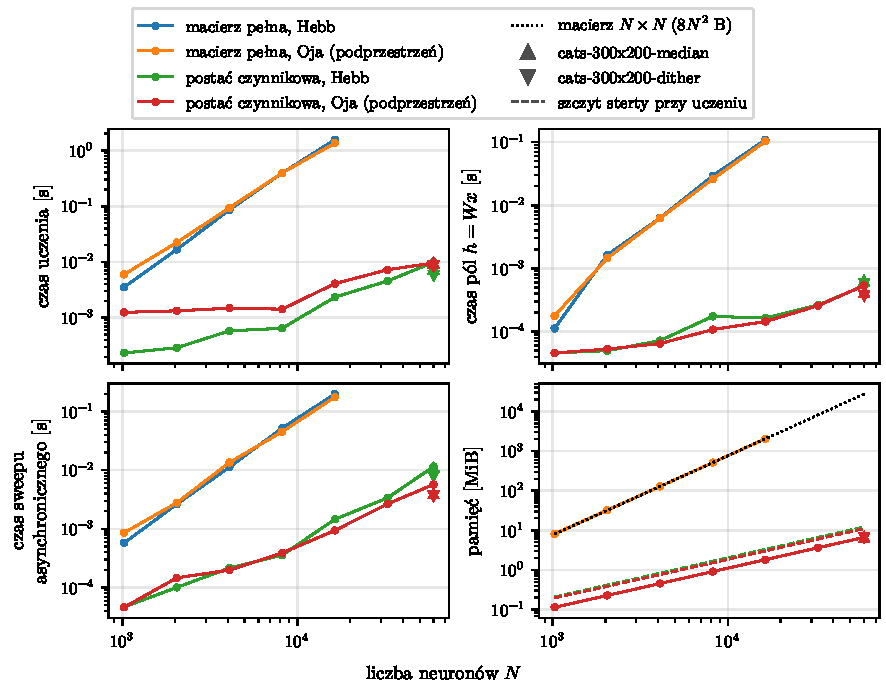
\includegraphics[width=0.8\textwidth]{benchmark/figures/benchmark.pdf}
    \caption{Czas uczenia, czas obliczenia pól $h = Wx$ dla wszystkich neuronów, czas kroku asynchronicznego i pamięć wag w zależności od liczby neuronów (skale logarytmiczne, mediany z 5 powtórzeń). Trójkąty oznaczają zbiory kotów.}
    \label{fig:benchmark}
\end{figure}

\noindent Wagi czynnikowe~\eqref{eq:wagi-czynnikowe} rosną liniowo z $N$ i przy $N = \num{60000}$ zajmują \qty{6.6}{MiB}. Szczyt pamięci przy uczeniu jest od \num{1.7} do \num{1.8} razy większy od rozmiaru wag. Uczenie trwa wtedy około \qty{10}{ms} dla obu reguł, także dla 356 epok reguły Oji, bo koszt epoki nie zależy od $N$ (rozdział~\ref{sec:uczenie}). Obliczenie pól wszystkich neuronów trwa około \qty{0.5}{ms}, a krok asynchroniczny na zdjęciach kotów trwa od \num{3.7} do \qty{11.0}{ms}.
